\documentclass[twoside,11pt]{article}

\usepackage{blindtext}

% Any additional packages needed should be included after jmlr2e.
% Note that jmlr2e.sty includes epsfig, amssymb, natbib and graphicx,
% and defines many common macros, such as 'proof' and 'example'.
%
% It also sets the bibliographystyle to plainnat; for more information on
% natbib citation styles, see the natbib documentation, a copy of which
% is archived at http://www.jmlr.org/format/natbib.pdf

% Available options for package jmlr2e are:
%
%   - abbrvbib : use abbrvnat for the bibliography style
%   - nohyperref : do not load the hyperref package
%   - preprint : remove JMLR specific information from the template,
%         useful for example for posting to preprint servers.
%
% Example of using the package with custom options:
%
% \usepackage[abbrvbib, preprint]{jmlr2e}

\usepackage{jmlr2e}

\usepackage{mathtools}
\usepackage{amsmath}  % use argmin + argmax, cf. https://tex.stackexchange.com/a/5255
\DeclareMathOperator*{\argmax}{arg\,max}
\DeclareMathOperator*{\argmin}{arg\,min}
\usepackage{bm}

\usepackage{enumitem}  % nested enumerations, cf. https://tex.stackexchange.com/a/126756

% Definitions of handy macros can go here

\newcommand{\dataset}{{\cal D}}
\newcommand{\fracpartial}[2]{\frac{\partial #1}{\partial  #2}}

% Heading arguments are {volume}{year}{pages}{date submitted}{date published}{paper id}{author-full-names}

\usepackage{lastpage}
\tabmlheading{WS 2024/25}{1-\pageref{LastPage}}{15.03.2025}{}{Simon Stürzebecher}

% Short headings should be running head and authors last names

\ShortHeadings{Interpretable Neural Networks using EAGGA}{Simon Stürzebecher}
\firstpageno{1}

\begin{document}

\title{Interpretable Neural Networks using EAGGA}

\author{\name Simon Stürzebecher \email simon.stuerzebecher@campus.lmu.de}

%\editor{My editor}

\maketitle

\begin{abstract}%   <- trailing '%' for backward compatibility of .sty file
  Tabular data proves to be difficult for neural networks, where they are still outperformed by other model classes.
  Following recent research, regularisation can improve their performance. Incorporating the EAGGA framework designed to
  enforce explainability, we improve interpretability and achieve performance comparable to that of XGBoost on the
  metrics AUC, number of features, number of pairwise interactions, and number of non-monotone feature effects.
  For this, we propose a sparse, regularised network architecture specifically suited for EAGGA's constraints on
  interaction and monotonicity.
\end{abstract}

\begin{keywords}
  tabular data, multi-objective optimization, interpretability, neural networks
\end{keywords}


\section{Introduction}
Regularisation has been extensively shown to improve performance from linear models to neural networks.
One of the most popular types of regularisation, Ridge or L2-regularisation is still the preferred method for handling
multicollinear data in linear models \citep[p. 55]{ridge}.
Practicioners training neural networks regularly use regularisation methods such as dropout to reduce
co-adaptation \citep[p. 1]{hinton2012improvingneuralnetworkspreventing} or early stopping to avoid overfitting on the training data \citep[p. 778f]{early_stopping}.
\\
Some regularisation can even increase interpretability, such as LASSO, or L1-regularisation for linear models, which reduces the number of
features used to fit the model by setting some coefficients to 0 \citep[p. 267]{lasso}.
\\
Neural networks as a model class have achieved impressive performance on a multitude of problems, yet still struggle with the most common format --
tabular data \citep[p. 7499]{Borisov_2024}.
Recent research, however, suggest that strong regularisation is beneficial to a neural network's performance on tabular data \citep[8]{NEURIPS2021_c902b497}.
\citet{EAGGA} propose a framework to increase the interpretability of XGBoost using regularisation.
In this report, we explore if the same framework can be extended to neural networks to tackle both interpretability and achieve performance on tabular data
that is on par with XGBoost.


\section{Background and Related Works}

\subsection{Interpretability}
As there is no clear definition for interpretability, we will consider it as ``the ability to provide \textit{explanations} in \textit{understandable terms} to a human'',
where \textit{explanations} are logical decision rules and \textit{understandable terms} relate to commonly used terms in the domain of the problem,
as suggested by \citet[chap. 1]{survey_NN_interpretability}. Further, we use the term ``explainability'' in an exchangeable manner with ``interpretability'',
as is commonly done.

% Why Interpretability is desirable?
Explainability of a model's reasoning is in many ways desirable. \citet[pp. 3-4]{Zach2019InterpretabilityOD} gives a range of examples,
amongst which are \textit{gaining trust}, e.g. when doctors rely on medical diagnosis predictions, avoiding \textit{subconcious biases} by
making sure loan approvals are non-discriminatory, or \textit{regulatory} reasons, most notably the EU's ``Right to Explanation'' warranted by the
GDPR \citep[p. 1]{review_NN_interpretability} or for approval of drugs discovered using machine learning models \citep[1B]{survey_NN_interpretability}.
It can further prove helpful for explaining unexpected drops in model performance, which could arise from optimizing a model with respect to loss and then judging its
performance on a different metric such as accuracy, a practice known as \textit{model debugging} \citep[1B]{survey_NN_interpretability} or for
\textit{scientific understanding} in domains where only models can make sense of increasingly complex data anymore and learnt knowledge encoded in a model needs to be
made accessible to humans to be used reliably \citep[p. 1]{review_NN_interpretability}.

Commonly, methods for model interpretation are divided into intrinsic methods, where the search space only comprises models with a structure simple enough to be
considered ``explainable'' (such as tree-based or simple linear models), and post-hoc methods, where interpretation methods are applied after model training.
Amongst post-hoc techniques, we can further divide the space into model-specific (such as analysing GLM coefficients) and model-agnostic
(e.g. partial depence plots, ALE) methods \citep[chap. 3.2]{molnar2022}.

% Taxonomy
\citet[chap. 2]{survey_NN_interpretability} extend this distinction to a three-dimensional taxonomy, allowing for better categorisation of neural networks (NNs),
a model class that in its fully-connected feedforwad form is inherently non-interpretable. % TODO: letztes halbsatz vllt lieber in intro unterbringen, hier ist der awkward und unnötig ausschmückend
\\
\textbf{Passive vs Active Approaches}, where \textit{passive} are all post-hoc methods and \textit{active} methods actively change either the architecture or
training process to increase model interpretability.
\\
\textbf{Type of Explanations}, distinguishing between \textit{example} methods, providing concrete examples of what leads to a desired output, \textit{attribution}
methods that attribute the effect on the output for a specific feature, \textit{hidden semantic} methods, which explain the types of inputs particular neurons or layers
pick up on, and logical \textit{rules}, such as if-then clauses or tree-induced rules.
\\
\textbf{Local vs Global Interpretability}, ranging from \textit{local} methods providing explanations based on individual samples, \textit{semi-local} methods,
explaining model behaviour for sets of samples grouped by some criterion, to \textit{global} methods, which explain the network as a whole.

% Evaluation
Given its unclear definition, evaluating interpretability can be challenging. \citet[3]{DoshiVelez2017TowardsAR} propose a taxonomy to categorise
possible evaluation methods based on their rigorousness.
\\
\textbf{Application-grounded evaluation} evaluates interpretations directly with respect to the task, by having human experts evaluate the outcome and
is therefore the most expensive and time-consuming of the three approaches.
\\
\textbf{Human-grounded metrics} is similar to application-grounded evaluation in that a human still evaluates the interpretations, but tries to simplify the task
so that a layperson can do it. Human-grounded approaches are especially suitable if it's sufficient to validate the general concepts of a task. A typical evaluation
set-up in this category is binary forced choice, where the human evaluator chooses, which of two generated explanations he prefers.
\\
\textbf{Functionally-grounded evaluation} is the least rigorous, but easiest to implement of the three. It assess explanatory quality according to some
formally defined proxy for interpretability and is particularly useful in ranking different models if their model-class is already identified
(e.g. via human-grounded evaluation) to be interpretable. The main challenge for functionally-grounded evaluation is finding a good proxy.

\subsection{Hyperparameter Optimization (HPO)}
In contrast to model parameters, which are optimized during training, hyperparameters (HPs) are those describing the machine learning algorithm and are
fixed before training. Because they usually have a significant impact on the trained model's performance, HPs are often optimized, too.
Let $\mathcal{D}\subseteq\mathcal{X}\times\mathcal{Y}$ be a dataset consisting of $n$
tuples drawn from the data-generating distribution, i.e. $(\boldsymbol{x}^{(i)}, y^{(i)})\stackrel{i.i.d.}{\sim}\mathbb{P}_{\boldsymbol{x}y},\forall i=1,...,n$.
Furthermore, let $\mathcal{I}:(\mathbb{D}\times\boldsymbol\Lambda)\rightarrow\mathcal{H}, (\mathcal{D},\boldsymbol\lambda)\mapsto\hat{f}$
be an algorithm that maps a given dataset $\mathcal{D}$ and HP configuration $\boldsymbol\lambda\in\boldsymbol\Lambda$ to a model $\hat{f}$.
Denote with $\mathcal{I}_{\boldsymbol\lambda}$ an algorithm with fixed HP configuration a chosen loss function with $L$.
The goal of model training is, for fixed $\boldsymbol\lambda$, to have $\mathcal{I}_{\boldsymbol\lambda}$ find model $\hat{f}$ minimising the expected generalisation error
$GE(\mathcal{I}_{\boldsymbol\lambda},\mathcal{D},L)=\mathbb{E}_{(\boldsymbol{x},y)\sim\mathbb{P}_{\boldsymbol{x}y}}[L(y,\mathcal{I}_{\boldsymbol\lambda}(\mathcal{D})(\boldsymbol{x}))]$
The goal of HPO, on the other hand, is to find $\boldsymbol\lambda$ minimising the expected generalisation error,
i.e. $\argmin_{\boldsymbol\lambda\in\boldsymbol\Lambda} GE(\mathcal{I}_{\boldsymbol\lambda},\mathcal{D},L)$.
For this, there is no analytical expression available, making HPO a blackbox optimization problem. \citep[pp. 2f]{10.1145/3610536}

We will first outline model-free methods to approach blackbox optimization problems, before presenting a model-based variant.

% model free
% grid + random search
The most basic model-free strategies for blackbox optimization are grid and random search.
In the latter, the user defines a range of interest for each HP and then evaluating points along a grid within the cartesian product of those.
This has the drawback of scaling extremely poorly in both number of HP dimensions and number of query points per range of interest.
Random search, on the other hand, randomly samples a value for each HP until it runs out of budget. Its explorative nature, ease of use, and no assumptions
about the model makes it a good baseline. It is also superior to grid search in cases were one or more HPs have little impact on model performance,
as for a given budget $B$, each HP will likely be queried with $B$ different values, whereas for grid search each HP will only be queried with $B^{1/N}$
different values for $N$ HPs. \citep[chap. 1.3]{feurer_hyperparameter_2019}

% evolutionary algorithms
Another popular class of model-free optimizers are evolutionary algorithms (EAs), which are conceptually simple and can handle even complex parameter spaces,
given appropriate implementation of operators.
EAs are iteratively evolving a population of individuals (an individual is simply a hyperparameter configuration) of size $\mu$, where in each iteration (generation),
$\lambda$\footnote{We distinguish between $\lambda\in\mathbb{N}$ when referring to the offspring size of EAs and $\boldsymbol\lambda\in\boldsymbol\Lambda$ when
referring to a hyperparameter configuration.} offspring are generated via three operators \citep[pp. 10-14]{genetic_algos}.
\\
\textbf{Reproduction} samples an individual from the population to reproduce with probability proportional to its fitnes. For HPO, fitness usually refers to the
performance metric the model resulting from the individual's HP configuration is evaluated on.
\\
\textbf{Crossover} selects two ``parents'' from the pool of reproducing individuals. An index $k$ is sampled at random and all HP values from
index $k$ on are swapped, yielding two new ``children'' individuals.
\\
\textbf{Mutation} randomly changes single HP values of an individual chosen for reproduction, e.g. by adding Gaussian noise to real values or flipping bits
on binary values.
\\
At the end of each generation, the EA keeps the best $\mu$ individuals, either only from the offspring (``$(\mu,\lambda)$-selection'') or more commonly from
population and offspring (``$(\mu+\lambda)$-selection''), which is also called an ``elitist'' strategy, as it's guaranteed to keep the best individual.
\citep[chap. 1.3]{feurer_hyperparameter_2019}

One of the most popular EA implementations is the ``Covariance Matrix Adaptation Evolution Strategy'' (CMA-ES).
It employs a multivariate normal distribution to generate offspring, for which the mean is a weighted average of the previous generation's individuals
and the covariance matrix similarly is the weighted covariance of the previous generation.
The weighing scheme for both is done in a way as to reproduce previously successful (i.e. selected) steps \citep[p. 8-11]{hansen2023cmaevolutionstrategytutorial}.

Another popular EA approach is Differential Evolution. Its populaton is randomly initialized so the entire search space is covered.
In each generation $g$, for each $\boldsymbol\lambda_{i,g}$ with $i=1,...,n$ it creates ``mutant vectors''
$\boldsymbol\nu_{i,g+1}=\boldsymbol\lambda_{r_1,g}+F\cdot(\boldsymbol\lambda_{r_2,g}-\boldsymbol\lambda_{r_3,g})$,
where $r_1,r_2,r_3\in\{1,...,n\}$ are mutually different random indices that also different from $i$ and $F\in[0,2]$ is constant.
For crossover, it then generates a ``trial vector'' $\boldsymbol\upsilon_{i,g+1}=(\upsilon_{i,g+1}^{(1)},\upsilon_{i,g+1}^{(2)},...,\upsilon_{i,g+1}^{(N)})^T$ with
\begin{equation}
  \upsilon_{i,g+1}^{(j)} = \begin{dcases}
    \nu_{i,g+1}^{(j)} & \text{if } u\le\text{CR}\text{ or } j=R \\
    \lambda_{i,g}^{(j)} & \text{else}
  \end{dcases}
\end{equation}
for a random index $R\in\{1,2,...,D\}$, sampled $u\sim U[0,1]$, and crossover constant $\text{CR}\in[0,1]$.
Selection is done by picking the better of $\boldsymbol\upsilon_{i,g+1}$ and $\boldsymbol\lambda_{i,g}$ with respect to fitness. \citep[p. 343]{differential_evolution}

% model based
Contrasting to model-free approaches, model-based methods fit a surrogate model on the target function and optimize the surrogate.
Currently, one of the most popular model-based approaches is Bayesian Optimization (BO).
BO is an iterative algorithm comprising a probabilistic surrogate model $\tilde{f}$ for the blackbox problem $f$ and an acquisition function.
It maintains and continually extends a set of points it already evaluated on the target function.
In each iteration, the posterior predictive distribution is determined by fitting the surrogate model on this set of points.
The acquisition function then retrieves the highest utility point from the surrogate model and evaluates it on the target function, after which it adds the point
to the set of queried points \citep[chap. 1.3.2]{feurer_hyperparameter_2019} and \citep[pp. 2f]{frazier2018tutorialbayesianoptimization}.
Evidently, neither the target function nor the surrogate model are optimized directly. Rather, the acquisition function trades-off exploration and exploitation of
the surrogate and is maximised to yield the next query point most likely to optimize the two objectives as defined by the acquisition function.
\\
Common choices for the acquisition function are Expected Improvement (Eq. \ref{eq-expected-improvement}) and Thompson Sampling (Eq. \ref{eq-thompson-sampling}).
\begin{equation}
  \text{EI}_t(\boldsymbol\lambda):=\mathbb{E}_t[(f(\boldsymbol\lambda)-f_t^*)^+]
  \label{eq-expected-improvement}
\end{equation}
\textbf{Expected Improvement} computes the expected minimisation over the incumbent $f_t^*$ for evaluating the target function $f$ at query point $\boldsymbol\lambda$.
$\mathbb{E}_t$ denotes the expectation under the posterior predictive distribution with $t$ query points, similarly, the current incumbent is the minimum value
of the target function from previous evaluations $(\boldsymbol\lambda_{1:t},f(\boldsymbol\lambda_{1:t}))$. \citep[p. 7]{frazier2018tutorialbayesianoptimization}
\begin{equation}  % TODO: take out
  f^{(t)}\sim\tilde{f}_t
  \label{eq-thompson-sampling}
\end{equation}
\textbf{Thompson Sampling}, on the other hand, can conceptually be described as drawing a candidate function $f^{(t)}$ from the posterior predictive distribution and
minimising it to obtain the next query point for the target function. \citep[p. 161]{7352306}
\\
Composing the other part of BO, surrogate models need to be able to model mean and variance of its target function estimate.
Commonly chosen models are Gaussian Processes (Eq. \ref{eq-gaussian-process}) and Random Forests.
\begin{equation}  % TODO: make inline or provide further information
  \text{GP}(m(\boldsymbol\lambda), k(\boldsymbol\lambda,\boldsymbol\lambda'))
  \label{eq-gaussian-process}
\end{equation}
\textbf{Gaussian Processes} (GP) are fully specified by their mean and covariance functions and have closed-form solutions.
The mean $m(\boldsymbol\lambda)$ fits all points already evaluated on the target function, while for the covariance or
kernel function $k(\boldsymbol\lambda,\boldsymbol\lambda')$ it is desirable that points close to
each other in HP space $\boldsymbol\Lambda$ exhibit stronger correlation than those far apart.
The kernel function can be freely chosen, a common choices is the Gaussian (Eq. \ref{eq-kernel-gaussian}) kernel with
hyperparameter $\alpha_0$. \citep[p. 5]{frazier2018tutorialbayesianoptimization}
\begin{equation}
  k(\boldsymbol\lambda,\boldsymbol\lambda')=\alpha_0 \exp(-\|\boldsymbol\lambda-\boldsymbol\lambda'\|_2^2)
  \label{eq-kernel-gaussian}
\end{equation}
A drawback of Gaussian Processes is its poor scalability in number of data points and number of hyperparameters, although there exist workarounds approximating the full GP
with only a subset of the samples. \citep[chap. 1.3.2]{feurer_hyperparameter_2019}
\\
\textbf{Random Forests}, unlike GPs, can handle complex hyperparameter spaces even including categorical and hierarchical HPs. Their computational complexity is also far
less, making them a popular alternative to Gaussian Processes. \citep[chap. 1.3.2]{feurer_hyperparameter_2019}

  
\subsection{Neural Architecture Search}
A special case of HPO is Neural Architecture Search (NAS). Because of the flexibility of neural network architectures (number of hidden layers, strength of dropout,
each layer can have a different numer of neurons, each layer can have a different activation function, etc.), traditional HPO methods cannot efficiently explore the
entire space.
In our extension of the EAGGA approach we don't employ NAS as research focusses on the NLP and image domains, % TODO: find some more references
where features (i.e. tokens or pixels, respectively) exhibit strong correlation amongst themselves, which is usually not the case for tabular data \citep[p. 7499]{Borisov_2024}.
Still, we want to outline two notable approaches for neural architecture search in this paper, one of which are \textbf{cell search spcaces}.
These modularise an NN into a chain-structure of cells, where each cell is a basic building block of the respective architecture. For regular feedforwad neural networks,
this could be a linear layer of fixed size and with a specific activation function,
for CNNs this could be a specific convolutional operation or pooling function, for instance.
Instead of tuning every hyperparameter, the sequential placement of the cells is then optimzed during NAS, e.g. via random search or Bayesian
Optimization. \citep[chap. 3.2]{elsken_neural_2019}
\\
Treating a neural network as a sequence of cells instead of one fixed entity further allows exploiting this structure with special sequential optimization techniques.
\citet[p. 3]{zoph2017neuralarchitecturesearchreinforcement} and \citet[pp. 2-4]{Zoph_2018_CVPR} propose a cell search method using RNNs and reinforcement learning.
The cells in their approach are not fixed, but have hyperparameters themselves, such as the filter size and the stride size of a convolutional layer.
These hyperparameters are then predicted sequentially, given all the already predicted hyperparameters of previous layers. The RNN is trained using reinforcement
learning, where the actions are the different values the network can predict for a given hyperparameter and the reward function is the RNN's performance on held-out
validation data.
\\
The second approach to NAS is the \textbf{one-shot model}, which trains a ``fabric'', which can be understood as a DAG comprising all architectures of a given
search space. Each path through the DAG is one specific network architecture, where the nodes represent a layer of neurons and the edges in-between are operations
on the layers' values. The entire DAG has one designated input and one output node.
It is then trained just like a regular NN, after which the optimal path, i.e. network architecture, is selected from the fabric.
This has the advantage of, albeit being slower than training a single model, being far more efficient and less expensive than training all architectures encoded
in the fabric. \citep[pp. 1-2, p.8]{saxena2017convolutionalneuralfabrics}
% don't necessarily talk about co-adaptation problem

\subsection{Multi-Objective Optimization}
In most applications, practicioners don't just want to optimize for performance exclusively but, for instance, also desire an interpretable model,
which they may measure via some proxy metric.
Let $c_1,c_2,...,c_m = \boldsymbol{c}:\boldsymbol\Lambda\rightarrow\mathbb{R}^m$ be the vector of $m$ objectives, the goal of multi-objective optimization (MOO)
is to minimise this vector \citep[p. 11]{10.1145/3610536}.

\subsubsection{Pareto-optimality}
Optimizing $\boldsymbol{c}$ usually comes with the challenge of conflicting objectives: improving one objective means deteriorating another.
We thus seek to find a set of trade-off solutions, so called \textit{non-dominated} points.
A point $\boldsymbol\lambda$ dominates another point $\boldsymbol\lambda'$ ($\boldsymbol\lambda\prec\boldsymbol\lambda'$) if there is no other point that is
strictly better in at least one objective and better or equal in the remaining ones. Formally,
\begin{equation}
  \forall i\in\{1,...,m\}:c_i(\boldsymbol\lambda) \le c_i(\boldsymbol\lambda') \wedge \exists j\in\{1,...,m\}:c_j(\boldsymbol\lambda) < c_j(\boldsymbol\lambda')
  \label{eq-pareto-domination}
\end{equation}
as defined in \citep[pp. 7f]{10.1145/3610536} and \citep[pp. 198f]{genetic_algos}.
\\
The set of non-dominated or \textit{Pareto-optimal}
points $\mathcal{P}:=\{\boldsymbol\lambda\in\boldsymbol\Lambda|\nexists\boldsymbol\lambda'\in\boldsymbol\Lambda\text{ s.t. }\boldsymbol\lambda'\prec\boldsymbol\lambda\}$
is commonly referred to as the \textit{Pareto set} and its image as the \textit{Pareto front}.
The goal of MOO is to find a set of non-dominated points $\hat{\mathcal{P}}$ approximating the true Pareto set $\mathcal{P}$ well.

% evaluation
There are different techniques to evaluate an estimated Pareto-front. If we have knowledge over the true Pareto-front, we can compute the distance between the approximation
and the true front. In most cases, this knowledge cannot be assumed.
Then, usually volume-based approaches are used for evaluation, most notably the hypervolume. The hypervolume, or S-metric, of a Pareto-front, computes the volume between
the estimated front and some chosen reference point, which is usually the worst point in objective space.
The larger the hypervolume, the closer the estimate is to the true Pareto-front. \citep[pp. 8-10]{10.1145/3610536}

\subsubsection{A-priori}
For optimizing a multi-objective problem, there are largely two general approaches.
One of those are \textit{a-priori} methods, of which we will briefly outline two popular techniques.

\textbf{Scalarization} approaches impose an implicit order of priority on the objectives.
The simplest one is optimizing a weighted sum of objective functions
\begin{equation}
  \argmin_{\boldsymbol\lambda\in\boldsymbol\Lambda} \sum_{i=1}^m w_i c_i(\boldsymbol\lambda)
  \text{ s.t. } \sum_{i=1}^m w_i=1 \wedge w_i>0,\forall i=1,...,m
  \label{eq-a-priori-scalarization-weighted-sum}
\end{equation}
Weights are chosen a-priori by the user and the solution is very sensitive to them, making this method very reliant on different
users' preferences. \citep[p. 11]{10.1145/3610536} and \citep[chap. 3.1]{NSGA}
\\
Another form of scalarization is the $\epsilon$-constraint, which translates all but one objective into constraints and then optimizes the remaining
objective subject to the constraints. Without loss of generality, the first constraint can be optimized
\begin{equation}
  \argmin_{\boldsymbol\lambda\in\boldsymbol\Lambda} c_1(\boldsymbol\lambda)
  \text{ s.t. } c_2(\boldsymbol\lambda)\le\epsilon_2,...,c_m(\boldsymbol\lambda)\le\epsilon_m
  \label{eq-a-priori-scalarization-epsilon}
\end{equation}
This method is, similarly to the weighted sum, conceptually simple yet also very sensitive to the chosen constraints. \citep[p. 12]{10.1145/3610536}
\\
Alternative to scalarization is the \textbf{lexicographic method}.
For it, the user assigns a priority to each objective and then greedily optimizes each objective in order of priority, constrained to the solutions of
the already optimized, higher-priority objectives. \citep[p. 13749]{lexicographic_MOO}
Again, solutions are very dependent on the user-defined priorisation.

\subsubsection{A-posteriori}
\label{sec-moo-post}
The disadvantage of a-priori methods is the missing knowledge of the interplay between a hyperparameter configuration and the trained model's
performance across objectives:
we can either restrict the search space to enforce some will, such as only using a maximum of 50\% of features, optimize for performance and use the
resulting model, or leave the search space unrestricted, adjust the loss function to incorporate all objectives and take its optimum.
In neither case do we know the impact our a-priori trade-off has on the final performance.
In practical applications, the impact on performance across all objectives is what matters.
This is the main advantage of a-posteriori methods: instead of implicitly defining a trade-off prior to training, we still evaluate multiple HP configurations
but keep the set of non-dominated solutions instead of just one that satisfies the trade-off criterion.
This is beneficial as it makes the relationship visible, a practicioner can now see, for instance, that a slight decrease in one objective might translate to
a significant improvement in another that would have been missed if the problem was optimized with a-priori methods.
\\
Aside from the usual baselines grid and random search there are multi-objetive Bayesian Optimization adaptations, mainly using one of two approaches:
\begin{enumerate}[label*=\arabic*.]
  \item Fitting a single surrogate model on scalarized objectives. \citet[pp. 54-56]{ParEGO} propose \textit{ParEGO}, which employs the augmented Tchebycheff function as
        scalarization to ensure the Pareto front is explored sufficiently.
  \item Fitting one surrogate per objective, then either 
  \begin{enumerate}[label*=\arabic*.]
    \item using one acquisition function per surrogate to return a set of promising candidate query points or
    \item using one overall acquisition function to aggregate the surrogates, such as \textit{EHI} as proposed by \citet[pp. 8f]{EHI}, which maximises
          the expected improvement of hypervolume.
  \end{enumerate}
\end{enumerate}

Lastly, there is also a multitude of multi-objective evolutionary algorithms (MOEA) to explore the Pareto front.
A key challenge for MOEAs is determining the fitness of an individual, as there are now multiple objectives that need to be incorporated instead of
one as in single-objective EA (SOEA).
We will outline the popular NSGA-II (Nondominated Sorting Genetic Algorithm II), which improves upon its predecessor NSGA \citep{NSGA} by making it
parameterless, ensuring elitism, and reducing the computational complexity of ranking of individuals \citep[p. 182]{NSGA_II}.
NSGA-II uses all the regular operators reproduction, mutation, and crossover that are already known from SOEA.
The difference is in the fitness function, which for NSGA-II comprises two parts: non-dominated sorting and crowding distance.
\\
\textit{Non-dominated sorting}, as described by \citet[p. 201]{genetic_algos} and \citet[pp. 183f]{NSGA_II} is an iterative procedure to ensure
elitist selection through ranking individuals by their fronts.
First, it assigns all individuals of the Pareto front a rank of 0. It then temporarily removes these individuals from the population and repeats
this procedure with an incremented rank number until no individuals are left.
\\
The second part, \textit{crowding distance} ensures sufficient diversity, i.e. exploration of the Pareto front.
The algorithm assigns each individual a score depending on how ``crowded'' the area in objective space around it is. Crowding distance is computed
as the mean side length of the cuboid spanned by its nearest neighbours as vertices in the objective space, where individuals without two neighbours
along some dimension are assigned an infinitely high distance value. The less the crowding distance, the more an area is by other individuals. \citep[p. 185]{NSGA_II}
\\
NSGA-II then ranks individuals by their non-dominated sorting front ranks in ascending order and by their crowding distance in descending order as tie breaker.
This ranking is then used for selecting the $\mu$ best individuals to keep for the next generation.
Reproduction follows a binary tournament selection, where two individuals are randomly drawn from the population and the better one according to the ranking gets
included in the reproduction pool for mutation and crossover.
\\
Conceptually, the reasoning behind using non-dominated sorting to rank individuals is intuitive: the closer an individuals front is to the Pareto front, i.e.
the smaller its front rank, the better it approaches the true Pareto front.
The usage of crowding distance, on the other hand, is not as straightforward. To understand it, we recall the goal of MOO, which is not merely optimizing
hypervolume, but to approximate the true Pareto front well.
Considering the scenario of only having individuals of one area in the objective space included in the Pareto front estimate makes it very unstable: removing this
area (i.e. the solutions from this area) would collapse the entire front estimate.
Considering now the opposite, having multiple areas making up the Pareto front estimate, makes it stable: removing one area would not impact the estimate a lot,
as it's still held up by other individuals. \citep[p. 185, pp. 189-192]{genetic_algos}
A possible proxy for exploration of the Pareto front is the hypervolume contribution. The hypervolume contribution of individual
$\boldsymbol\lambda\in\hat{\mathcal{P}}$ is the difference between the hypervolume of the entire estimated Pareto front vs the hypervolume of the front without the
individual: $\text{CON}_{\hat{\mathcal{P}}}(\boldsymbol\lambda)=\text{HYP}(\hat{\mathcal{P}})-\text{HYP}(\hat{\mathcal{P}}\setminus\{\boldsymbol\lambda\})$,
where $\text{HYP}(\hat{\mathcal{P}})$ denotes the hypervolume induced by the Pareto set $\hat{\mathcal{P}}$ \citep[p. 384]{10.5555/1943267.1943271}.


%likely shouldn't be an entire section
\section{EAGGA}
\label{sec-eagga}
EAGGA, as proposed by \citet{EAGGA}, is an NSGA-II inspired algorithm that optimizes performance along with three interpretability objectives.
The three interpretability proxies are
\begin{itemize}
  \item NF: the relative number of features used in the model
  \item NI: the relative number of pairwise interaction effects in the model
  \item NNM: the relative number of non-monotone feature effects in the model
\end{itemize}
The authors argue that a sparse model as indicated by a low NF score helps interpretability by reducing the number of e.g. ALE plots necessary in post-hoc
analysis \citep[p. 540]{EAGGA}. Similarly, a low NI score reduces the interplay between features and thus the dimensionality of post-hoc analysis plots
and a low NNM avoids complex non-monotone feature effects, which is often desirable in practical use-cases such as loan approval, where a higher income should
translate to a higher chance of approval.
Lastly, performance is measured by the area under the receiver operating characteristic curve (AUC), which trades-off the true against the false positives rate.
\\
\citet[pp. 540f]{EAGGA} acknowledge that this set-up creates the complex ``extended search space'' $\check{\boldsymbol\Lambda}$ to be optimized over, containing
tuples $(\boldsymbol\lambda, \boldsymbol{s}, \boldsymbol{I}_s, \boldsymbol{m}_{\boldsymbol{I}_{\boldsymbol{s}}})=\check{\boldsymbol\lambda}\in\check{\boldsymbol\Lambda}$
with
\begin{itemize}
  \item $\boldsymbol\lambda\in\boldsymbol\Lambda$ being the model's hyperparameter configuration
  \item $\boldsymbol{s}\in\{0,1\}^p$ being a binary vector denoting which features are used in the model
  \item $\boldsymbol{I}_s\in\{0,1\}^{p\times p}$ being a binary matrix denoting included pairwise interactions between features
  \item $\boldsymbol{m}_{\boldsymbol{I}_{\boldsymbol{s}}}\in\{-1,0,1\}^p$ being the vector denoting the monotonicity constraint of a feature (-1 decreasing, 0 none, 1 increasing)
\end{itemize}
Consequently, the optimization problem over this space would be
\begin{equation}
  \argmin_{\check{\boldsymbol\lambda}\in\check{\boldsymbol\Lambda}} \big(
    GE(\mathcal{I}_{\check{\boldsymbol\lambda}},\mathcal{D}),
    NF(\hat{f}_{\mathcal{D},\check{\boldsymbol\lambda}}),
    NI(\hat{f}_{\mathcal{D},\check{\boldsymbol\lambda}}),
    NNM(\hat{f}_{\mathcal{D},\check{\boldsymbol\lambda}})
  \big)
  \label{eq-eagga-extended-space}
\end{equation}
The authors thus introduce the equivalence relation $R$ ``allowed to interact'' on the set of features $C$. They further denote all features included in the model with $C_s$.
This induces a group structure of equivalence classes, where features allowed to interact belong to the same class and share the same monotonicity attribute.
Using this group structure, they define a much simpler ``augmented serach space'' $\tilde{\boldsymbol\Lambda}=\boldsymbol\Lambda\times\mathcal{G}$ comprising of
the cartesian product of the model hyperparameter space $\boldsymbol\Lambda$ and the group structure space $\mathcal{G}$.
Each group structure $\boldsymbol{G}\in\mathcal{G}$ consists of $g$ groups:
\begin{itemize}
  \item $G_1=C\setminus C_s$ being the set of excluded features
  \item $G_k=(E_k,M_{E_k}), \forall k=2,...,g$ being tuples with
  \begin{itemize}
    \item $E_k\subseteq C_s$ being the set of features in group $k$, i.e. features allowed to interact with each other
    \item $M_{E_k}$ being the monotonicity constraint of group $k$
  \end{itemize}
\end{itemize}
To generate new offspring, they use a regular evolutionary algorithm on the model hyperparameters $\boldsymbol\Lambda$ and a grouping genetic algorithm (GGA) on
the group structure space $\mathcal{G}$, with adapted mutation and crossover operators.
The authors further introduce a special initialization of the group structures to increase the sample-efficiency of their algorithm compared to random initialization.
\citep[pp. 541-543]{EAGGA}


\section{Extension to Neural Networks}
EAGGA as implemented by \citet{EAGGA} applies the optimizer to XGBoost, which proved to vastly outperform a union of competitor models with respect to
dominated hypervolume and achieved comparable or better performance than ParEGO optimizing over the
extended search space $\check{\boldsymbol\Lambda}$ \citep[pp. 543-545]{EAGGA}.
Our work extends EAGGA to neural networks. We chose this model class for several reasons:
\begin{enumerate}[label*=\arabic*.]
  \item NNs are notoriously uninterpretable due to complex transformations of the feature space
  \item Non-linear activation functions implicitly model interactions without direct control of which features interact with each other
  \item There are no monotonicty guarantees in neural networks
\end{enumerate}
The optimizer is implemented largely as described by \citet{EAGGA} with only minor changes due to there being no straightforward transferability of some functions
from R to Python or differences in model properties between XGBoost and neural nets.\\

\subsection{Architectural Details}
We implement the group structures as described by \citet[p. 541]{EAGGA} with an additional list encoding whether the signs of individual features should
be inverted (-1) or not (1), as detected by the monotonicity detector.
The features included in the group structure are then passed to a custom pytorch Dataset implementation, which outputs only the included features, multiplied with their
individual sign. This allows the groups' monotonicity constraints to be encoded with only $\{0,1\}$, as proposed by \citet[p. 543]{EAGGA}.
The entire group structure is then passed to the neural network, where the architecture is built accordingly.
\begin{figure}
  \centering
  \includegraphics[width=\linewidth]{./architecture.png}  % scale figure, cf. https://tex.stackexchange.com/a/16584
  \caption{TODO: caption}
  \label{fig-nn-architecture}
\end{figure}
\\
Applying EAGGA to NNs requires defining a special architecture to realise interaction and monotonicity constraints.
The neural network consists of a group of fully-connected sub-networks that are not connected amongst each other, as visualised in Figure \ref{fig-nn-architecture}.
Each equivalence class in the group structure has its own sub-network, so that it is guaranteed that only the features within that group can interact with each other.
\\
For the hidden layers, we use ReLU activations with dropout afterwards, after which a shared output layer transforms the concatenated output of the sub-networks
to a probability using the Sigmoid activation function.
We use AdamW with default parameters, optimizing a binary cross-entropy loss with Sigmoid implicit in the loss function for better numerical stability. The network
itself thus outputs only a ``logit'', which is the pre-activation output in pytorch.
\\
Feature sparsity is achieved by only training on the included features that are passed to the network from the dataset.
\\
Grouping the network into sub-networks enables restricting feature interactions to only those features that are included in the respective group.
The $\max$-operation in the ReLU induces a certain interaction effect on its inputs. It is important to note that this is a different kind of interaction
than the multiplicative one known, for instance, from the linear model.
Given a layer's input $\boldsymbol{x}$ and without loss of generality omitting the bias, the ReLU activation is defined as follows
\begin{equation}
  \text{ReLU}(\boldsymbol{x})=\max(0,\sum_{j=1}^p w_j x_j)
  \label{eq-our-extension-interaction-1}
\end{equation}
We see that the interaction is not of the form $x_j \cdot x_{j'}$ but rather of a form where the sum $w_j x_j+w_{j'} x_{j'}$ decides whether $x_j,x_{j'}$
pass through the activation or not.
In other words, the interaction is given by the fact that
\begin{equation}
  \max(0,w_j x_j + w_{j'} x_{j'})\neq\max(0,w_j x_j)+\max(w_{j'} x_{j'})
  \label{eq-our-extension-interaction-2}
\end{equation}
Finally, monotonicty is achieved by clipping the respective sub-network's weights to $[0,\infty)$ after each epoch. Whether a feature's effect is
increasing or decreasing depends on the individual feature's sign encoded in the custom dataset implementation.
Consider the vector form computation of a pre-activation hidden neuron $\boldsymbol{o}_{\text{in}}^{(l)}\in\mathbb{R}^{p^{(l)}}$ of layer $l$
\begin{equation}
  \boldsymbol{o}_{\text{in}}^{(l)}=\boldsymbol{W} \boldsymbol{o}_{\text{out}}^{(l-1)} + \boldsymbol{b}
  \label{eq-our-extension-monotonicity}
\end{equation}
where $\boldsymbol{o}_{\text{out}}^{(l)}$ denotes the value of layer $l$ after applying ReLU, $\boldsymbol{W}\in\mathbb{R}^{p^{(l)} \times p^{(l-1)}}$ refers to
the weight matrix and $\boldsymbol{b}\in\mathbb{R}^{p^{(l)}}$ to the bias.
A function $f$ is monotonically increasing if and only if $\forall x_1\le x_2$ it holds that $f(x_1)\le f(x_2)$ and thus
$\boldsymbol{W} \boldsymbol{o}_{\text{out}}^{(l-1)} + \boldsymbol{b}$ is clearly only monotonically increasing if and only if
$\boldsymbol{W}\in\mathbb{R}_{0+}^{p^{(l)}\times p^{(l-1)}}$, where $\mathbb{R}_{0+}=[0,\infty)$.
Therefore, $\boldsymbol{o}_{\text{out}}^{(l)}=\text{ReLU}(\boldsymbol{o}_{\text{in}}^{(l)})=\max(0,\boldsymbol{o}_{\text{in}}^{(l)})$ is a monotonically increasing
function if and only if the weights are clipped as described. Bias clipping is not necessary as it is a constant additive term.


\subsection{Overall Algorithm}
Our NNs use the following hyperparameters initialized as described
\begin{itemize}
  \item Total number of layers $\in\{3, ..., 10\}$, initialized from a truncated Geometric distribution with $\pi=0.5$.
        This includes input and output layers, the number of hidden layers is thus $\in\{1, ..., 8\}$
  \item Number of nodes per hidden layer $\in\{3, ..., 20\}$, initialization from a truncated Geometric distribution with $\pi=0.5$
  \item Dropout probability $\in[0, 1]$, initialized from a truncated Gamma distribution with shape 2 and scale 0.15
\end{itemize}
For the group structure initialization we also employ feature, interaction, and monotonicity detectors.
\\
The feature detector is as described by \citet[p. 542]{EAGGA}, but instead of fitting ten trees and using the relative number of features as
probability for the truncated Geometric distribution, we use a constant value of 0.5, as the sklearn DecisionTree examination is not straightforward.
Further, in preliminary experiments we found the sampled number of features to occassionally be larger than the number of non-zero values in the
normalised information gain filter. This can happen if the former is equal to the total number of features and one or more features are independent form the
target. In these edge cases we use all features with non-zero filter-values instead.
\\
The interaction detector similarly uses a constant probability of 0.5 to sample the number of interactions to be used instead of the relative number of interactions
from ten decision trees, for the same reasoning as for the feature detector. Also, for the FAST algorithm, when computing the interaction scores we don't
use the residual sum of squares but the mean accuracy, as the datasets all have binary targets and FAST thus fits a logistic instead of a linear regression.
\\
The monotonicty detector is implemented as described by \citet[p. 543]{EAGGA}, using the default decision tree hyperparameters from mlr3 in Python.
\\
Both the models in the interaction and the monotonicity detector (FAST and an ensemble of decision trees, respectively) use 80\% of the data for model estimation and
the remaining 20\% to compute their scores.


\subsection{Experimental Setup}
\begin{figure}
  \centering
  \includegraphics[width=\linewidth]{./dataset_split.png}
  \caption{TODO: caption}
  \label{fig-dataset-split}
\end{figure}
We evaluate our models just like \citet[pp. 543f]{EAGGA} by computing the dominated hypervolume along AUC, NF, NI, NNM with reference point $(0, 1, 1, 1)^T$.
Internally, this is implemented as minimising $1-\text{AUC}$ and a reference point $(1, 1, 1, 1)^T$.
For NF, we simply count the relative number of included features.
NI sums the numbers of all possible pairwise interactions in each group ${p_k \choose 2}$ and divides them by the number of all possible pairwise interactions
on the entire dataset ${p \choose 2}$.
NNM counts the relative number of features in unconstrained equivalence classes.
\\
Our dataset is split as visualised in Figure \ref{fig-dataset-split}.
We apply an outer holdout train-test split with 1/3 of the dataset being held for final testing, the 2/3 are used for 5-fold cross-validated training of each individual,
as described by \citet[p. 543]{EAGGA}.
What is different for our implementation is that on each training portion of the CV split, we further apply a holdout split, where 80\% are used for model training and
20\% are reserved for early stopping.
\\
We use a conservative early stopping stratetgy, where each fold is always trained for a minimum of 200 epochs, keeping track of the fold's model with the lowest loss.
After 200 epochs, our criterion with a patience of 100 epochs is applied: now, if the current epoch's model loss is greater than the mean of the last 100 epochs'
losses, training in this fold stops early and returns the model with the lowest loss over the entire fold's training period.
If no early stopping is triggered, we train each fold for a maximum of 10 minutes and return the model with the lowest loss on the early stopping portion.
\\
The model is then evaluated on the remaining portion from the CV split and after each generation, we keep the best $\mu=100$ individuals and generate $\lambda=10$
offspring for the next generation and repeat this for 8 hours.
\\
The final evaluation of the individuals from the cross-validated Pareto set is then conducted on the held 1/3 of the dataset. Each individual
is trained on the 2/3 training portion for the maximum number of epochs the individual required in the cross-validated training.
Oftentimes, for cross-validation with early stopping, the final model is only trained on the mean or median number of epochs from CV.
We decided specifically on the maximum after examining the loss over epochs in preliminary experiments, as plotted in Figure \ref{fig-es-losses}
for the final experimental setup. Those show that there is no uptick in losses on the early stopping portion indicating that training too long does not increase
the validation error.
\\
We trained in Sagemaker Notebooks on AWS and did initial training runs on
ml.g4dn.xlarge\footnote{2 vCPUs, 16GiB RAM, 1 NVIDIA T4, cf. \url{https://aws.amazon.com/ec2/instance-types/g4/}} instances with CUDA.
There was, however, no noticeable speed-up in model training compared to the much more economical
ml.t3.medium\footnote{2 Intel Xeon 8000 vCPUs, 4GiB RAM, cf. \url{https://aws.amazon.com/ec2/instance-types/t3/}} instances, after which we decided to run the
final experimental setup on those.
\\
In total, we run our models on the same datasets as \citet[p. 544]{EAGGA}, except for the 2 largest ones ``philippine'' and ``gina'' (308 and 970 features, respectively),
as those ran out of memory when initializing the interaction effects.
\\
In rare cases (anecdotally once every ~10 datasets), we observed our monotonicity detector generating a group monotonicty attribute of -1, which crashed the computation.
For these cases, we implemented a function to import a previous generation of individuals to be able to pick up from where the training crashed and not train anew.
This happened once for the dataset ``madeline'' after generation 9 and training for 5 hours 45 minutes, and hence we imported the generation and ran it for the remaining
2 hours 15 minutes.


\section{Experimental Results and Discussion}

% have two figures next to each other
\begin{figure}
  \centering
  % make figure wider than textwidth: https://tex.stackexchange.com/a/16584
  \makebox[\textwidth][c]{\begin{minipage}{0.6\linewidth}
      \centering
      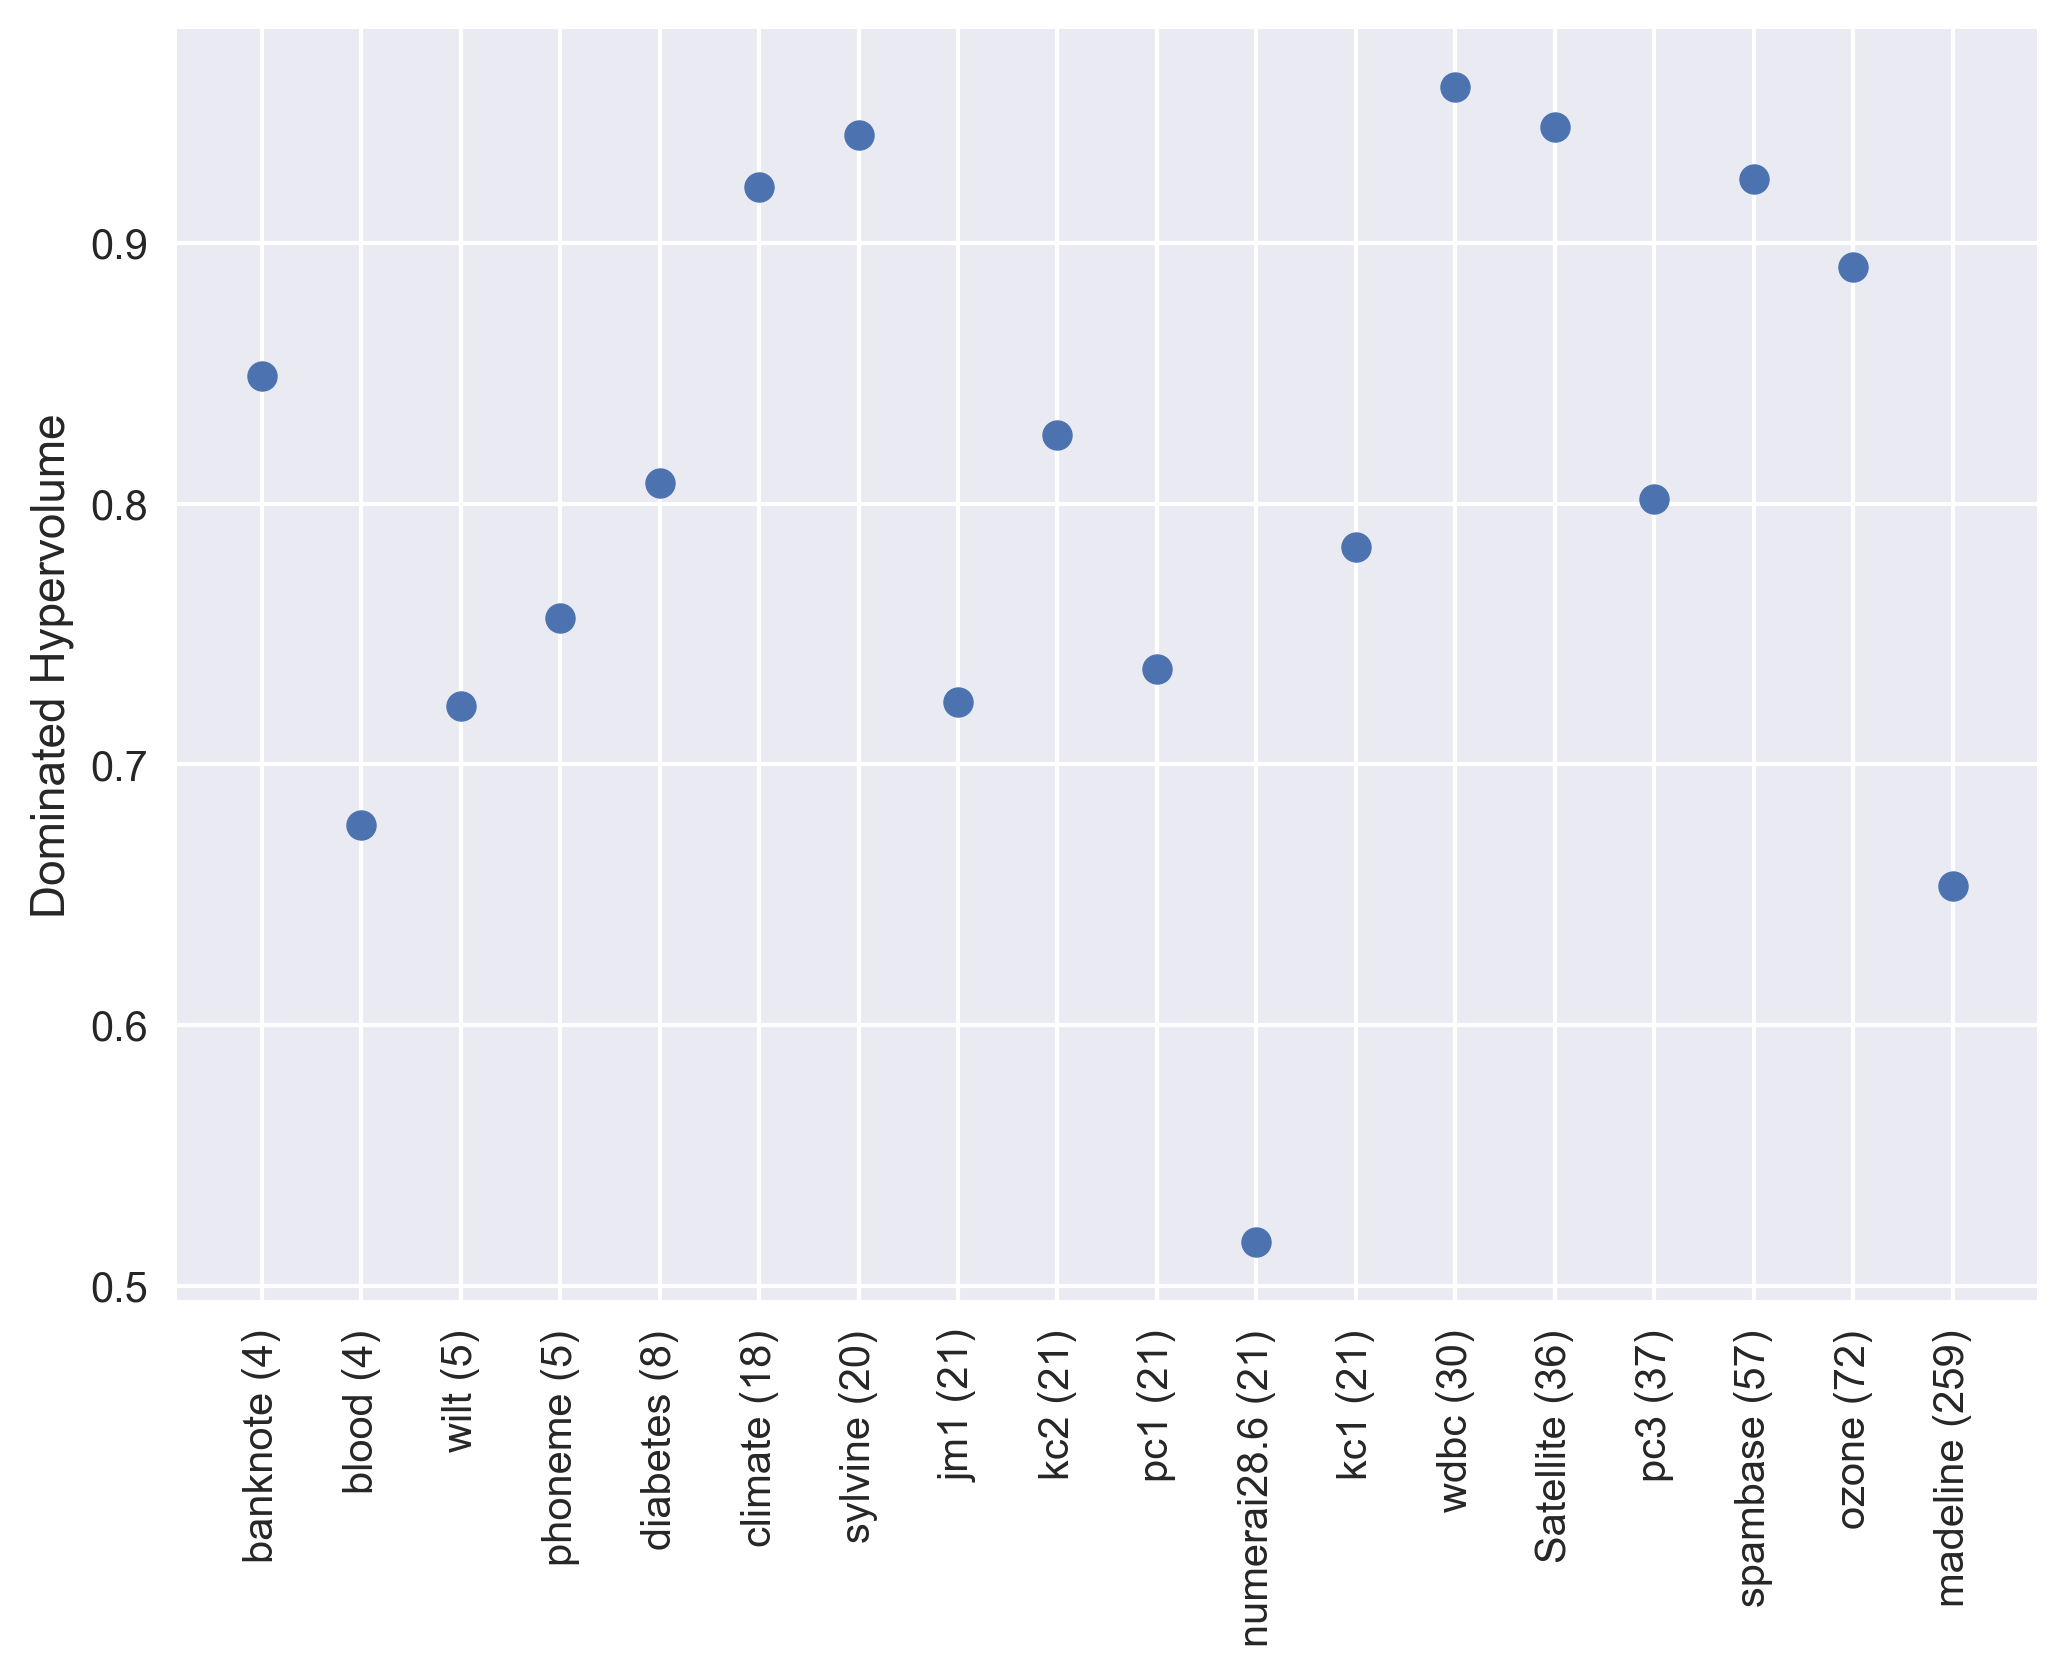
\includegraphics[width=\linewidth]{../code/export/plot_test_dhvs.png}
      \caption{Dominated Hypervolume of NNs trained using XGBoost.}
      \label{fig-test-dhvs}
  \end{minipage}\hfill
  \begin{minipage}{0.6\linewidth}
      \centering
      \includegraphics[width=\linewidth]{./EAGGA-XGB-dhv.PNG}
      \caption{Mean dominated Hypervolume of $EAGGA_{\text{XGBoost}}$, $EAGGA_{\text{XGBoost}_{\text{md2}}}$, and union of competitors averaged over
      10 replications. Bars represent standard errors. \citep[Figure 2, p. 544]{EAGGA}}
      \label{fig-eagga-xgb-dhvs}
  \end{minipage}}
\end{figure}
As evident from Figures \ref{fig-test-dhvs}, \ref{fig-eagga-xgb-dhvs}, applying EAGGA to neural networks yields comparable performance to applying it to XGBoost,
both with and without restricting the maximum tree depth.
A direct comparison to unrestricted neural networks trained with regular stochastic gradient descent has not been made, as this would have led to a hypervolume of 0
due to NF, NI, and NNM all being 1.
Similar to $EAGGA_{\text{XGBoost}}$ and $EAGGA_{\text{XGBoost}_{\text{md2}}}$, our extension consistently outperforms the union of competitors.
Unfortunately, due to time constraints, we were not able to compare the performance against a union of competitors including an unrestricted neural network
instead of XGBoost, although we hypothesise that, given unrestricted NNs' struggle on tabular data compared to XGBoost, the outperformance over the union would
be even greater.
\\
Examining the Pareto sets returned from training, which are accessible on our GitHub repository\footnote{\url{https://github.com/simon29st/ws2425-tab-ml/}}
at ~/code/export/*.csv, we can observe a clear trend in the
Pareto sets' models' hyperparameters:
\begin{itemize}
  \item the total number of layers is mostly 3 or 4, but goes as high as 7 for the Satellite (36) and diabetes (8) datasets
  \item the nodes per hidden layer are mostly in the range between 3 and 6, but go as high as 12 on the diabetes (8) dataset
  \item the dropout probability goes as high as 0.7 on the climate (18) and spambase (57) dataset, but is mostly in the 0.1 to 0.3 range
\end{itemize}
The returned group structures are more diverse:
NF goes up to 1 for individuals in the Pareto sets of phoneme (5) and blood (4). Further datasets with low feature cardinality exhibt similarly high
NF scores, with bankote (4) up to 0.75, climate (18) up to 0.67, and diabetes (8) up to 0.5. For the remainder, NF is much lower. The heightened NF for
datasets with less features can be a possible consequence of shorter training times: on average, low feature cardinality datasets train quicker and thus
for more generations than high cardinality datasets. This in turn means that their group structure space is far more likely to be exhaustively searched,
with then most of the performance improvements coming from changes to the model's hyperparameters.
As a consequence of the consistently low NF (except for low cardinality datasets), NI and NNM are equally very low, as they are directly dependent on the
number of features included in the model.
\\
The contributions to the dominated hypervolumes are predominately low for the models in the Pareto set, often being below 0.1, with the most contribution
often coming from the featureless learner. This is a sign for good and stable exploration of the Pareto front, as outlined in Section \ref{sec-moo-post}
\\
The loss graphs in Figure \ref{fig-es-losses} suggest that some models could have benefitted from longer training on some datasets, as some losses have not
coverged when the early stopping criterion was triggered.
This indicates that the criterion was likely triggered by a short-term spike, which could potentially be resolved by not comparing the current epoch's loss
to the mean of the previous 100 epochs but, for instance, the mean of a range of more recent epochs to the last 100.
This strategy, on the other hand, would then likely yield to even longer training periods on those datasets that clearly have converged, as evident by
horizontal loss graphs.
As the loss graphs remain horizontal and there is no uptick again, this would likely not be detrimental to model performance and the main ``risk'' would be
more a expensive computation from longer trainings.
\\
The AUC used in computing the dominated hypervolume over generations in Figure \ref{fig-val-dhvs} is the mean AUC over all folds on the validation set.
All but 3 datasets, 2 of which were only trained for 1 generation, exhibit improvement of their dominated hypervolume over generations. The absolute as
well as relative improvement, however, is almost negligible, suggesting there to be no large decrease in dominated hypervolume, would we have just evaluated
the group structure initialized by the detectors.
This was also the reason behind not running EAGGA on the philipine and gina datasets on randomly initialized detectors (as the detectors for those datasets
ran out of memory due to the high feature cardinality), as the detectors prove vital for the initial performance. This finding is also in
line with \citep[Fig. 4, p. 545]{EAGGA}.
\\
Clearly, there are some artifacts causing drops along the y-axis in most plots. This is likely due to the inconsistent computation of the Pareto front
by a third-party library: in preliminary experiments we observed slightly varying front ranks on a synthetic sample of 10 (AUC, NF, NI, NNM) vectors.
Unfortunately, this behaviour was still present when switching to another library for front rank computation, and thus not fixable for us.
From our anecdotal evidence, the variations in rankings in these preliminary experiments only concerned few samples that were assigned to alternating
neighbouring fronts, hence we considered it tolerable.
\\
Another observation from the logs during training is AUC occassionally being less than 0.5.
In general, AUC can then simply be inverted, as the model can usually always simply predict the opposite.
In our case, however, this is not possible as easily due to weight clipping for groups with a monotonicty constraint.
A potential scenario were an AUC less than 0.5 could happen is when AdamW has high momentum, leading to negative weights that are then clipped to the
non-negative domain at the end of the epoch.
We acknowledge that weight clipping is a very imperfect way of enforcing monotonicity, but currently seems to be the only way to implement this type of
constrained optimization in pytorch.

% belongs in "general algorithm"
%    - preliminary
%  * our implementation of feature + interaction detectors likely tend to include
%    - more features + interactions for high p datasets
%    - less for low p datasets
%    - remember: original paper samples \# of features included from truncated geometric distribution, what is not mentioned is probability of this distribution
%      is determined from fitting 10 trees + looking at relative \# of features used (cf. their github repo ~/R/TunerEAGGA.R function get\_n\_selected\_rpart())
%    -> mlr3 default decision tree max depth 30
%      * i.e. datasets with p < 30 might use all features, which translates to trunc geom prob = 1
%      * vice-versa for p >> 30 datasets relative \# features < 0.5 (our trunc geom prob)
%      * similar reasoning for pairwise interactions

\section{Conclusion and Future Outlook}
% Conclusion
The EAGGA framework has been shown to be able to preserve performance while increasing interpretabiltiy of XGBoost models on tabular data, which has long been 
a challenging discipline for neural networks. Following recent research suggesting that regularisation can improve NN performance on
tabular data \citep[8]{NEURIPS2021_c902b497}, we extend EAGGA \citep{EAGGA} to neural networks, utilising its regularising properties to achieve similar
performance with neural networks as with XGBoost and simultaneously increase interpretability of this notoriously uninterpretable model class.
As a consequence, we propose a new architecture allowing to model the equivalence relations of the EAGGA framework.
We create a model whose interpretation is active, attributional, and global in the framework of \citet[chap. 2]{survey_NN_interpretability}, and find
overall performance, as measured on the dominated hypervolume of (AUC, NF, NI, NNM) to be comparable to that of XGBoost fitted using EAGGA.
\\

% Future Outlook
Due to the low sample-efficiency of evolutionary algorithms, a multi-objective Bayesian Optimization variant on the augmented search space
(refer Section \ref{sec-eagga}) could deliver the strongest training time improvement.
There are two avenues to explore this, either via a change to the surrogate model or by adapting the acquisition function.
A surrogate model using a custom computed prior with high values and no uncertainty in unfeasible regions and regular uncertainty in feasible regions could be a solution.
An unfeasible region is for instance one, where a feature is in multiple equivalence classes, or where two features in the same equivalence class have opposing
monotonicity constraints.
The second option, adapting the acquisition function, may prove to be computationally less complex for datasets with many features.
This would mean using an unrestricted surrogate model and then taking account the constraints in the acquisition function. Similar approaches have been
tried on unrelated problems by \citep{10.5555/3020751.3020778} and \citep{perrone2019constrainedbayesianoptimizationmaxvalue}.


% Manual newpage inserted to improve layout of sample file - not
% needed in general before appendices/bibliography.


\vskip 0.2in
\bibliography{references}


\appendix
\section{Software used}
for implementation we used
openml \cite{OpenML}, \cite{OpenMLPython},
numpy \cite{numpy},
pandas \cite{pandas1}, \cite{pandas2},
pytorch \cite{PyTorch},
scikit-learn \cite{scikit-learn},
scipy \cite{SciPy},
pymoo \cite{pymoo}, and
tqdm \cite{tqdm}

\section{Plots}
\begin{figure}
  \centering
  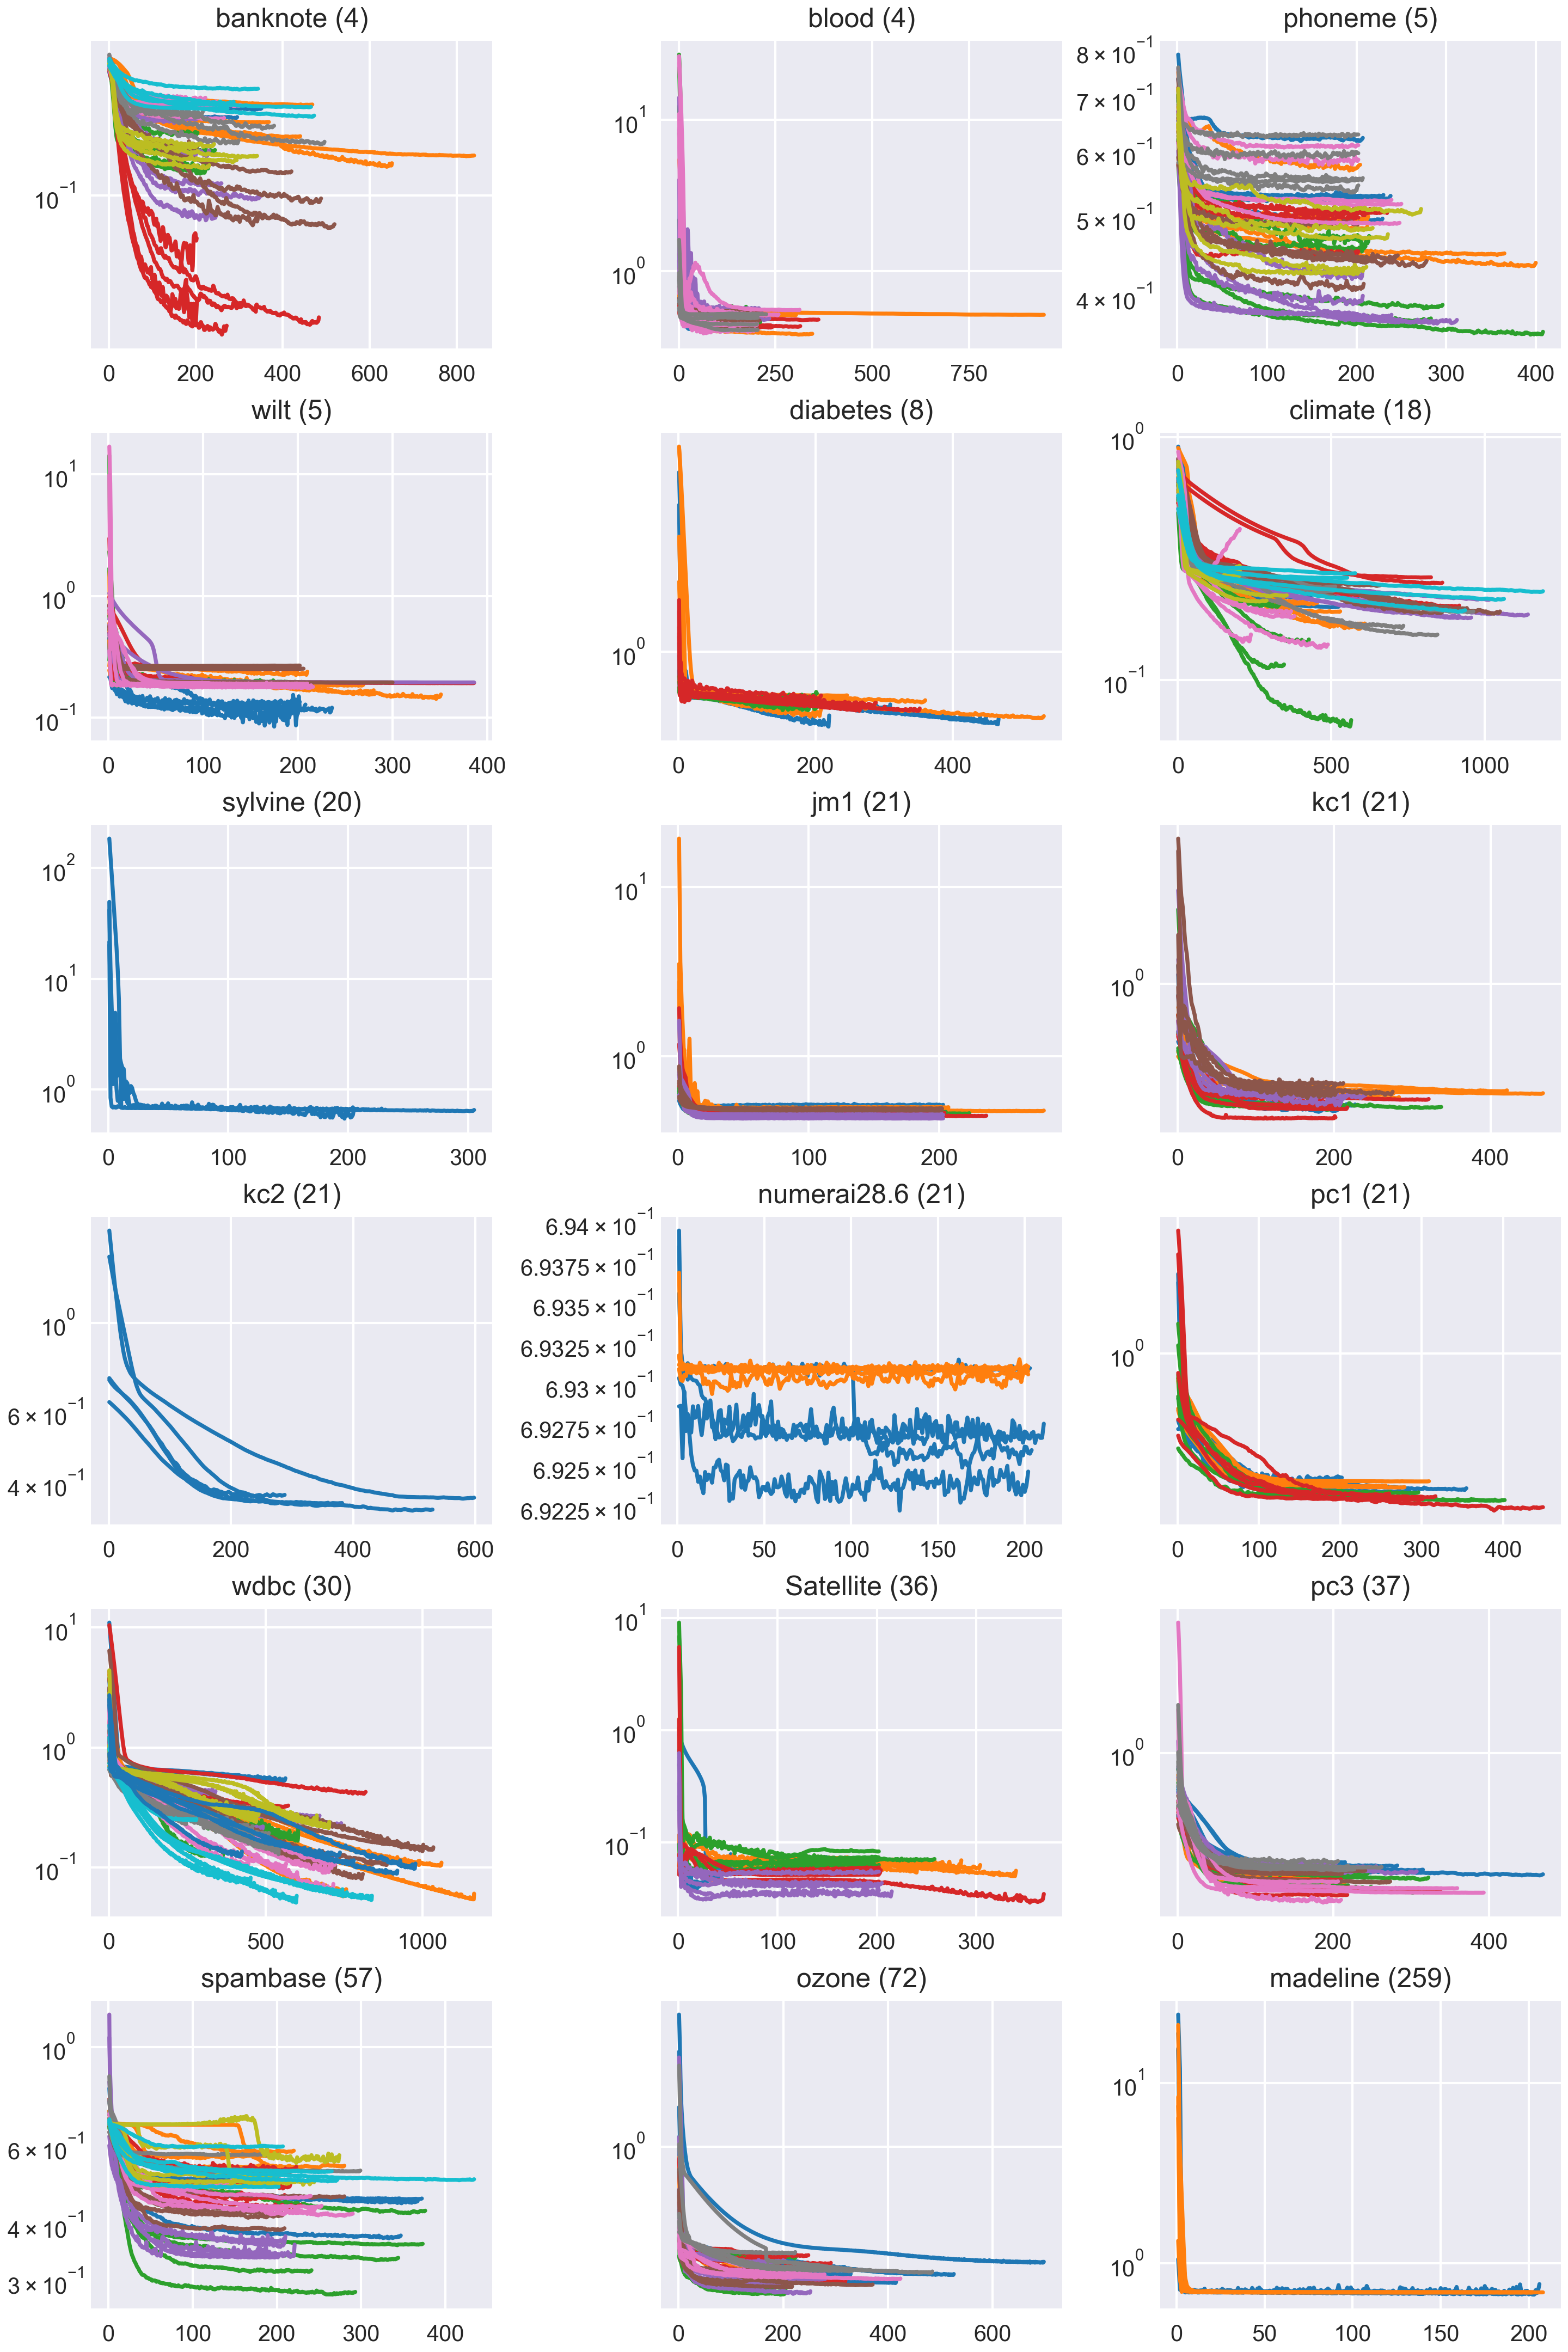
\includegraphics[width=0.9\linewidth]{../code/export/plot_early_stopping_losses_pareto_set.png}
  \caption{Pareto set loss of all datasets, evaluated on early stopping set. Same colours denote losses coming from folds of the same individual.
            x-axes portrait epochs, y-axes binary cross entropy loss.}
  \label{fig-es-losses}
\end{figure}

\begin{figure}
  \centering
  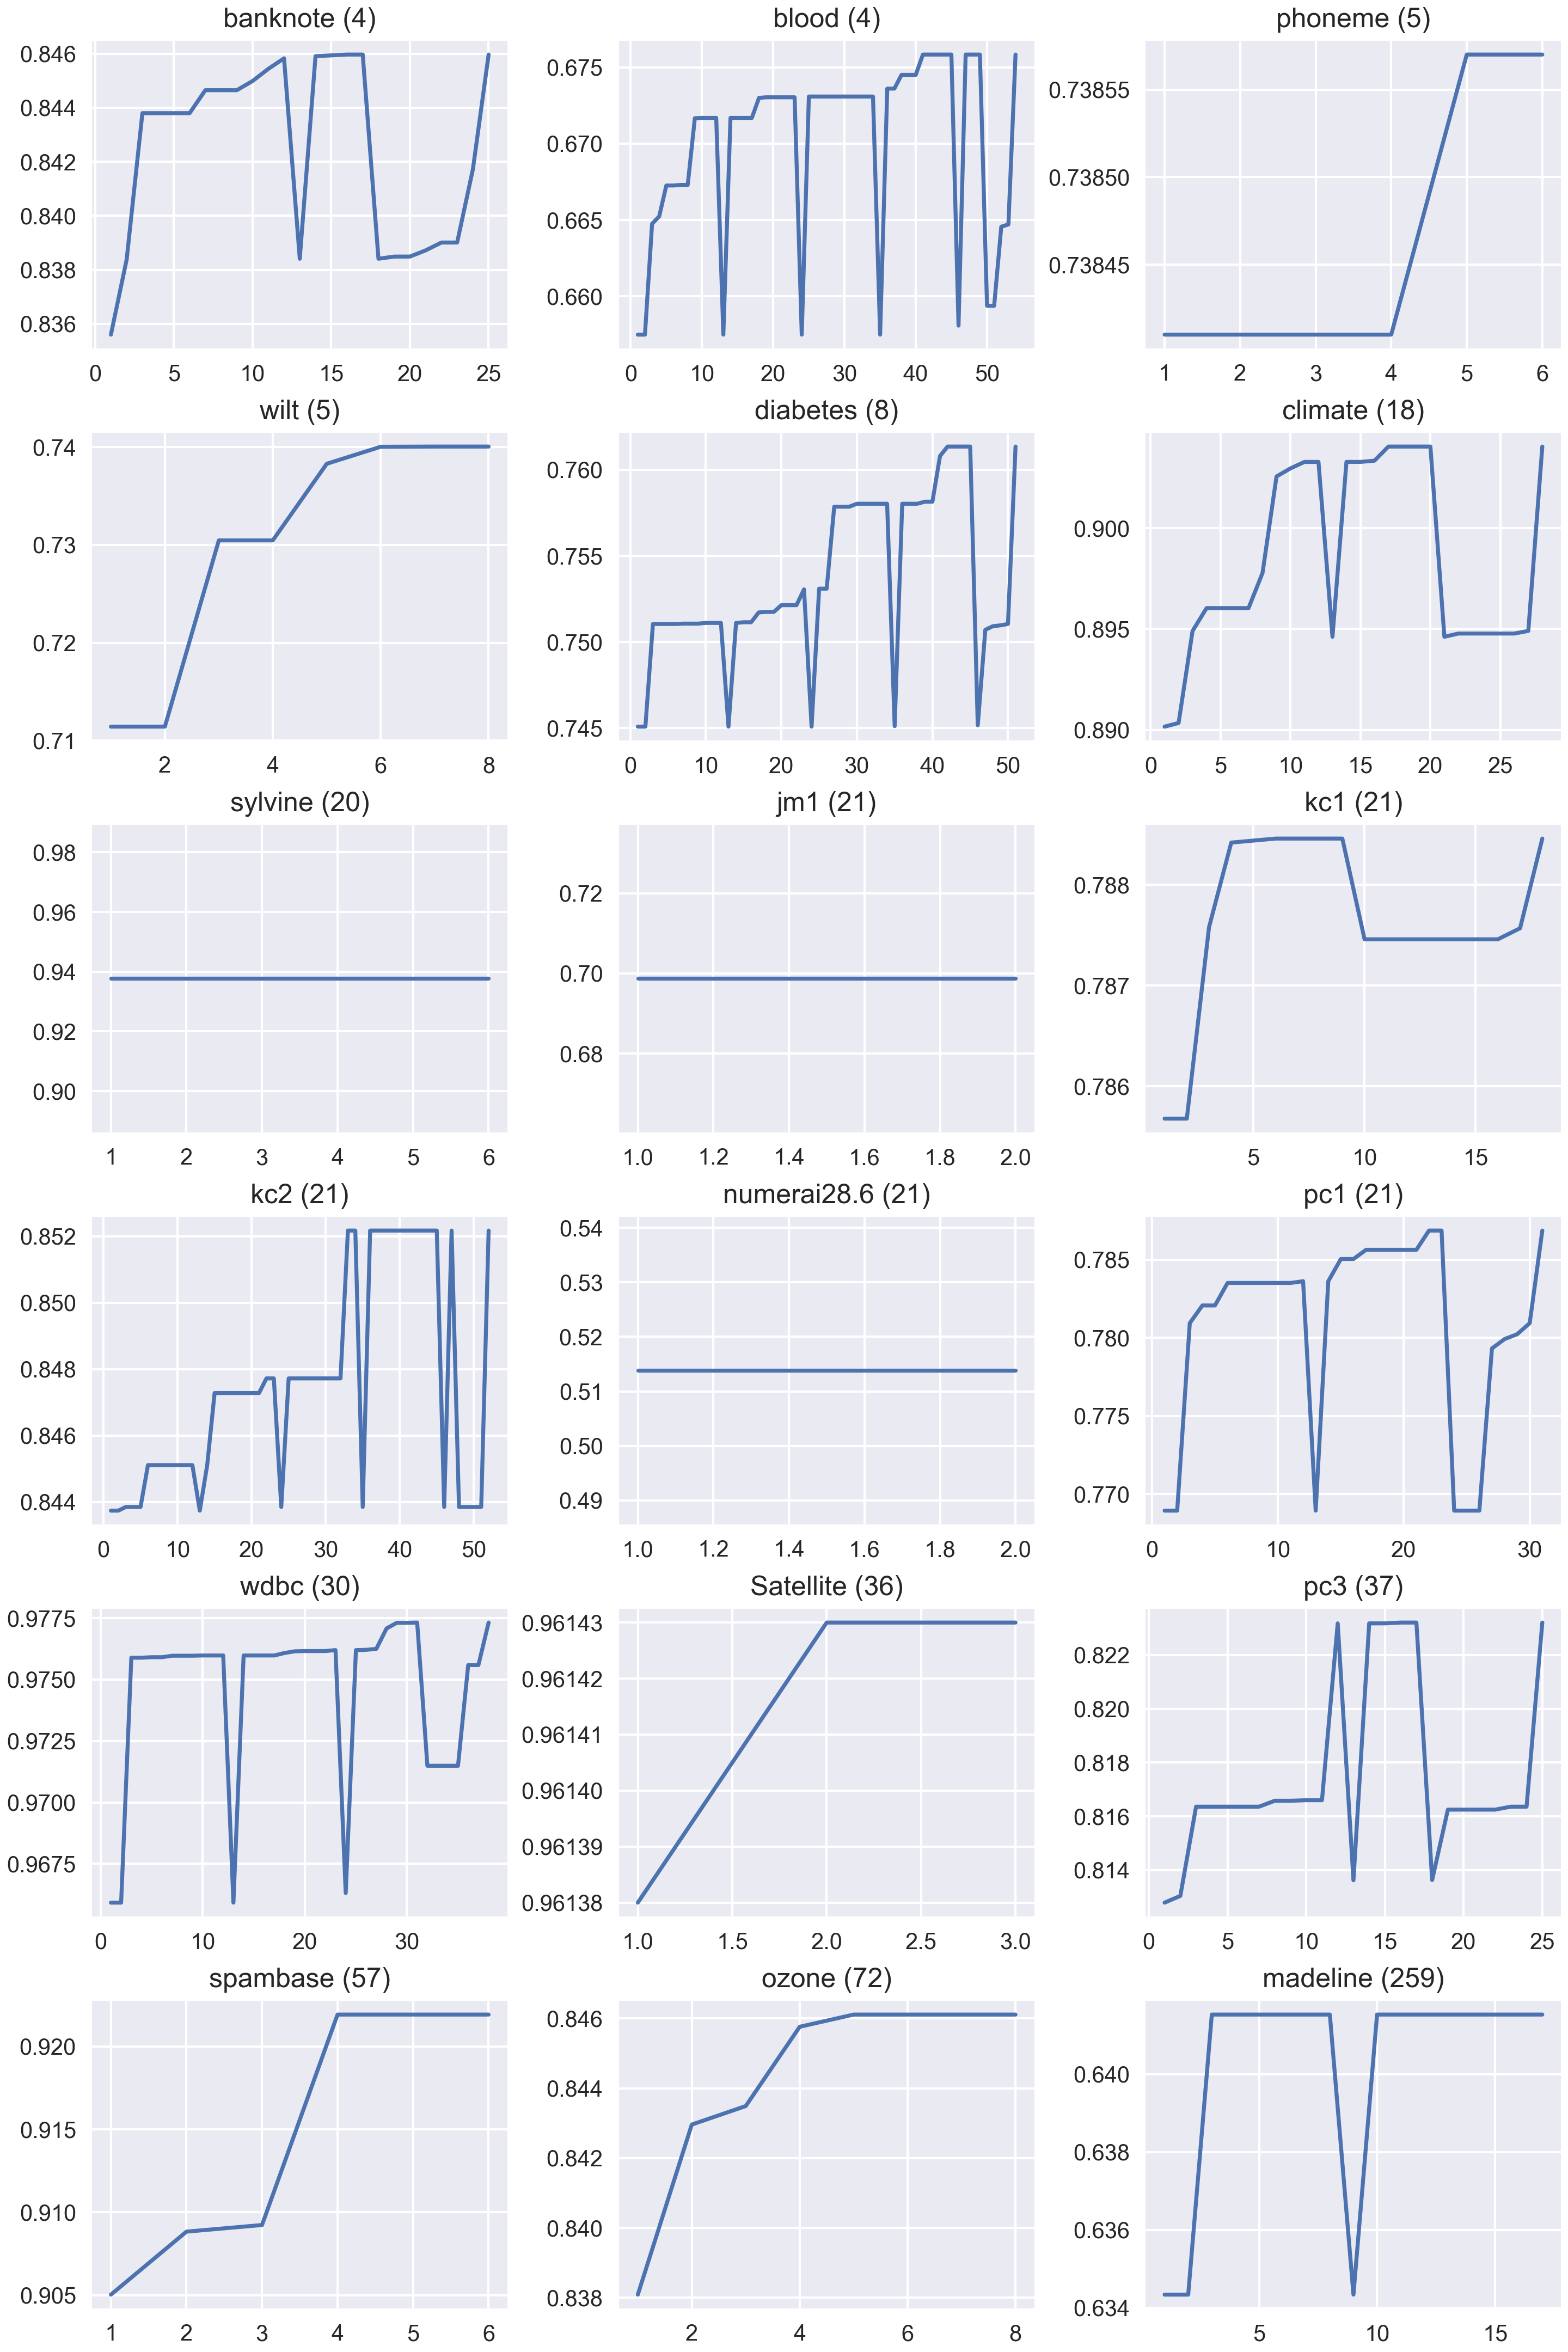
\includegraphics[width=0.9\linewidth]{../code/export/plot_val_dhvs_over_time.png}
  \caption{Dominated hypervolume over generations, evaluated on validation set.
            x-axes portrait generations, y-axes dominated hypervolume using mean AUC over folds.}
  \label{fig-val-dhvs}
\end{figure}

\end{document}
